\documentclass{article}

\usepackage{GOST}
\usepackage[T1, T2A]{fontenc}
\usepackage[utf8]{inputenc}
\usepackage[russian]{babel}
\usepackage{cmap}
\usepackage{amssymb}
\usepackage{amsmath}
\usepackage{hyperref}

\usepackage{listings}
% Для листинга кода:
\lstset{ 
	language=C,                 % выбор языка для подсветки (здесь это С)
	basicstyle=\small\sffamily, % размер и начертание шрифта для подсветки кода
	numbers=left,               % где поставить нумерацию строк (слева\справа)
	numberstyle=\tiny,           % размер шрифта для номеров строк
	stepnumber=1,                   % размер шага между двумя номерами строк
	numbersep=5pt,                % как далеко отстоят номера строк от подсвечиваемого кода
	showspaces=false,            % показывать или нет пробелы специальными отступами
	showstringspaces=false,      % показывать или нет пробелы в строках
	showtabs=false,             % показывать или нет табуляцию в строках
	frame=single,              % рисовать рамку вокруг кода
	tabsize=2,                 % размер табуляции по умолчанию равен 2 пробелам
	captionpos=t,              % позиция заголовка вверху [t] или внизу [b] 
	breaklines=true,           % автоматически переносить строки (да\нет)
	breakatwhitespace=false, % переносить строки только если есть пробел
}


\graphicspath{{images/}}

\linespread{1.5}

\title{Отчет по анализу алгоритмов}
\date{2020}
\author{Pavel Khetagurov}

\begin{document}
	\begin{table}[ht]
	\centering
	\begin{tabular}{|c|p{400pt}|} 
	\hline
		\begin{tabular}[c]{@{}c@{}} 
\includegraphics[scale=0.15]{EmblemBMSTU} \\\end{tabular} &
		\footnotesize\begin{tabular}[c]{@{}c@{}}\textbf{Министерство~науки~и~высшего~образования~Российской~Федерации}\\\textbf{Федеральное~государственное~бюджетное~образовательное~учреждение}\\\textbf{~высшего~образования}\\\textbf{«Московский~государственный~технический~университет}\\\textbf{имени~Н.Э.~Баумана}\\\textbf{(национальный~исследовательский~университет)»}\\\textbf{(МГТУ~им.~Н.Э.~Баумана)}\\\end{tabular}  \\
	\hline
	\end{tabular}
\end{table}
\noindent\rule{\textwidth}{4pt}
\noindent\rule[14pt]{\textwidth}{1pt}
\hfill 
\noindent
\makebox{ФАКУЛЬТЕТ~}%
\makebox[\textwidth][l]{\underline{~~~~«Информатика и системы управления»~~~~~~~~~~~~~~~~~~~~~~~~~~~~~~~~~~~~~~~~~~~~}}%
\\
\noindent
\makebox{КАФЕДРА~}%
\makebox[\textwidth][l]{\underline{~~~~~~~«Программное обеспечение ЭВМ и информационные технологии»~~~~~~~~}}%
\\


\begin{center}
	\vspace{3cm}
	{\bf\huge Отчёт\par}
	{\bf\Large по лабораторной работе №7\par}
	\vspace{0.5cm}
\end{center}


\noindent
\makebox{\large{\bf Название:}~~~}
\makebox[\textwidth][l]{\large\underline{~Поиск в словаре~~~~~~~~~~~~~}}\\

\noindent
\makebox{\large{\bf Дисциплина:}~~~}
\makebox[\textwidth][l]{\large\underline{~Анализ алгоритмов~~~~~~~~~~~~~~~~~~~~~~~~~~~~~~~~~~~~~~~~~~~~~~~~~~~~}}\\

\vspace{1.5cm}
\noindent
\begin{tabular}{l c c c c c}
    Студент      & ~ИУ7-55Б~               & \hspace{3.5cm} & \hspace{3.5cm}                 & &  Хетагуров П.К \\\cline{2-2}\cline{4-4} \cline{6-6} 
    \hspace{3cm} & {\footnotesize(Группа)} &                & {\footnotesize(Подпись, дата)} & & {\footnotesize(И.О. Фамилия)}
\end{tabular}

\vspace{1cm}

\noindent
\begin{tabular}{l c c c c}
    Преподователь & \hspace{6cm}   & \hspace{3.5cm}                 & & Л.Л. Волкова \\\cline{3-3} \cline{5-5} 
    \hspace{3cm}  &                & {\footnotesize(Подпись, дата)} & & {\footnotesize(И.О. Фамилия)}
\end{tabular}

\begin{center}	
	\vfill
	\large \textit {Москва, 2020}
\end{center}

\thispagestyle {empty}
\pagebreak
	\newpage
	\tableofcontents
	\newpage
	\begin{center}
	    \section*{Введение}
	\end{center}
	\addcontentsline{toc}{section}{Введение}
		\indent В данной лабораторной работе будет рассмотрена система конвеерной обработки.
	\newpage
	\section{Аналитическая часть}
	В данном разделе будут поставлены цели и задачи работы, будут рассмотренны основные теоритические сведения связанные с алгоритмами сортировки.
		\subsection{Цель и задачи работы}
			\textbf{Цель работы:} Научиться работать с потоками и разделяемыми ресурсами.
			\newline 
			\indent \textbf{Задачи работы:}
			\begin{enumerate}
				\item разработать систему из трех последовательных очередей, выполняющихся в отдельных потоках;
				\item реализовать разработанную систему;
				\item провести эксперимент, показывающий параллельное наступление событий.
			\end{enumerate}

		\subsection{Организация взаимодействия потоков}
		Так как потоки выполняются в общем адресном пространстве необходимо обеспечить корректное обращение к разделяемой памяти. Одним из способов достигнуть этого является мьютекс.
		\newline
		\indent Мьютекс (от mutual exclusion — «взаимное исключение») — примитив синхронизации, обеспечивающий взаимное исключение исполнения критических участков кода \cite{mutex}.
		
	\subsection{Вывод}
	В данной части были поставлены задачи и цель работы, рассмотрено взаимодействие потоков, понятие мьютекса.
	\newpage
	\section{Конструкторская часть}
		В данном разделе будут рассмотренны схемы алгоритмов, требования к функциональности ПО.
		\subsection{Требования к ПО} 
		ПО должно иметь один режим работы, в котором производится демонстрация работы. На вход системы подаются N элементов. В результате работы программы выводятся все события, произошедшие в системе, отсортированные в порядке наступления. Каждая очередь должна работать в своем потоке и завершать свою работу после обработки N элементов.	 	
		\subsection{Описание системы}
		Система состоит из трех очередей, последовательно соединенных между собой. В первую очередь генератором записываются входные данные, а из последней очереди данные попадают в результирующий массив. Во время входа и выхода из очереди, ставится временная метка.
		\newline
		\indent Между очередями находятся некоторые обработчики, обрабатывающие очередной элемент из предыдущей очереди и записывающие его в следующую. Причем время обрабатывания элемента должно быть больше времени диспетчирезации.
	\subsection{Вывод}
	В данном разделе были рассмотрена реализуемое ПО и обозначены требования к нему.
	
	\newpage
	\section{Технологическая часть}
	Ниже будут представлены средства реализации и листинги реализованной программы.
	\subsection{Средcтва реализации}
	Выбранный язык программирования - Golang, так как он предоставляет удобные средства для парралелизма -  goroutines \cite{go}. Среда разработки - Visual Studio \cite{vs}.
\newline
	\indent Технические характеристики машины, на которой проводились тесты:
	\begin{itemize}
	\item Windows 10 x64;
	\item 8 ГБ оперативной памяти;
	\item CPU: AMD FX(tm)-6350 Six-Core Processor 3.90GHz;
	\item 6 логических ядер.
	\end{itemize}	
	\subsection{Реализации алгоритмов}
	Ниже представлены листинги реализованной программы.
	На листинге \hyperref[mainLst]{[\ref{mainLst}]} представлен файл main.go.
	\begin{lstlisting}[label=mainLst, caption=main.go]
package main

import (
	"fmt"
	"sync"
	"time"

	queue "aa/lab_05/queue"
)

const MAX_ELEMENT = 100

var wg sync.WaitGroup
var log []string
var mutexLog sync.Mutex

type SetTimestamp func(*queue.Element, int64)

func pingPlace(id int, message string, time int64) {
	go func() {
		mutexLog.Lock()
		log = append(log, fmt.Sprintf("%d     %s    %d", id, message, time))
		mutexLog.Unlock()
	}()
}

func doStuff(milliseconds int) {
	time.Sleep(time.Millisecond * time.Duration(milliseconds))
}

func startHandle(queueFirst *queue.Queue, milliseconds int) {
	defer wg.Done()
	for i := 0; i < MAX_ELEMENT; {
		element := new(queue.Element)
		element.ID = i
		queueFirst.Mu.Lock()
		queueFirst.Push(element)
		queueFirst.Mu.Unlock()
		timeNow := time.Now().UnixNano()
		queue.SetFI(element, timeNow)
		pingPlace(element.ID, fmt.Sprintf("  Insert %d  ", 1), timeNow)
		doStuff(milliseconds)
		i++
	}
}

func handleQueue(firstQueue *queue.Queue, secondQueue *queue.Queue, stLeave SetTimestamp, stIn SetTimestamp, queueNumber int, milliseconds int) {
	defer wg.Done()
	for i := 0; i < MAX_ELEMENT; {
		firstQueue.Mu.Lock()
		element := firstQueue.Pop()
		firstQueue.Mu.Unlock()
		if element != nil {
			timeNow := time.Now().UnixNano()
			stLeave(element, timeNow)
			pingPlace(element.ID, fmt.Sprintf("  Leave %d   ", queueNumber), timeNow)
			doStuff(milliseconds)
			secondQueue.Mu.Lock()
			secondQueue.Push(element)
			secondQueue.Mu.Unlock()
			timeNow = time.Now().UnixNano()
			stIn(element, timeNow)
			pingPlace(element.ID, fmt.Sprintf("  Insert %d  ", queueNumber+1), timeNow)
			i++
		}
	}
}

func main() {
	firstQueue := queue.Queue{}
	secondQueue := queue.Queue{}
	thirdQueue := queue.Queue{}
	answerQueue := queue.Queue{}

	wg.Add(1)
	go handleQueue(&firstQueue, &secondQueue, queue.SetFO, queue.SetSI, 1, 300)
	wg.Add(1)
	go handleQueue(&secondQueue, &thirdQueue, queue.SetSO, queue.SetTI, 2, 600)
	wg.Add(1)
	go handleQueue(&thirdQueue, &answerQueue, queue.SetTO, queue.SetA, 3, 300)
	wg.Add(1)
	go startHandle(&firstQueue, 100)

	wg.Wait()

	for i := 0; i < len(log); i++ {
		fmt.Println(log[i])
	}
}
	\end{lstlisting}
		На листинге \hyperref[queueLst]{[\ref{queueLst}]} представлен файл queue.go.
	\begin{lstlisting}[label=queueLst,caption=queue.go]
package queue

import (
	"sync"
)

type Element struct {
	ID                 int
	TimestampFirstIn   int64
	TimestampFirstOut  int64
	TimestampSecondIn  int64
	TimestampSecondOut int64
	TimestampThirdIn   int64
	TimestampThirdOut  int64
	TimestampAnswer    int64
}

func SetFI(this *Element, timestamp int64) {
	this.TimestampFirstIn = timestamp
}

func SetFO(this *Element, timestamp int64) {
	this.TimestampFirstOut = timestamp
}
func SetSI(this *Element, timestamp int64) {
	this.TimestampSecondIn = timestamp
}
func SetSO(this *Element, timestamp int64) {
	this.TimestampSecondOut = timestamp
}
func SetTI(this *Element, timestamp int64) {
	this.TimestampThirdIn = timestamp
}
func SetTO(this *Element, timestamp int64) {
	this.TimestampThirdOut = timestamp
}
func SetA(this *Element, timestamp int64) {
	this.TimestampAnswer = timestamp
}

type Queue struct {
	Mu    sync.Mutex
	Array []*Element
}

func (this *Queue) Push(element *Element) {
	this.Array = append(this.Array, element)
}

func (this *Queue) Pop() (element *Element) {
	if len(this.Array) > 0 {
		element = this.Array[0]
		this.Array = this.Array[1:]
	}
	return
}

	\end{lstlisting}
	\subsection{Вывод}
	В данном разделе были описаны программные и аппаратные средства реализации, были представлены листинги программы.

	\newpage
	\section{Экспериментальная часть}
	В данной главе будет представлен пример работы программы и продемонстрировано параллельное наступление событий.
	\subsection{Пример работы программы}
	Пример работы программы представлен на рисунке \hyperref[programmWork]{[\ref{programmWork}]}
	 	\begin{figure}[h!]
		 	\center{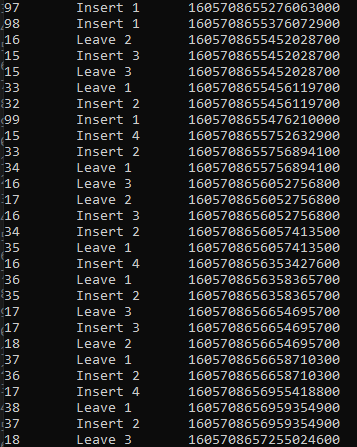
\includegraphics[scale=0.9]{programmWork.png}}
		 	\caption{Пример работы программы}
		 	\label{programmWork}
	 	\end{figure}
	
	
	\subsection{Вывод}
	Как видно из вывода программы, события выполнялись параллельно. 

	\newpage
	\begin{center}
		\section*{Заключение}
	\end{center}
	\addcontentsline{toc}{section}{Заключение}
	\indent \indent В данной лабораторной работе была разработана система конвееров, работающих с разделяемыми ресурсами, она были реализована, а также было показана параллельность выполнения конвееров. Цель работы достигнута, все задачи выполнены.
	\newpage
	\addcontentsline{toc}{section}{Список литературы}
	
	\begin{center}
	\begin{thebibliography}{3}
	\bibitem{mutex}
	Mutex. Wikipedia [Электронный ресурс]. Режим доступа: (дата обращения - 18.11.2020) Свободный. URL: https://en.wikipedia.org/wiki/Lock\_(computer\_science)
	\bibitem{go}
	Golang [Электронный ресурс]. Режим доступа: (дата обращения - 18.11.2020) Свободный. URL: https://golang.org/
	\bibitem{vs}
	Visual Studio [Электронный ресурс]. Режим доступа: (дата обращения - 18.11.2020) Свободный. URL: https://visualstudio.microsoft.com/ru/

	\end{thebibliography}
	\end{center}
\end{document}